\section{Control Algorithm}\label{sec:abstract-description}
\subsection{Block Diagram}\label{subsec:block-diagram}
\begin{center}
    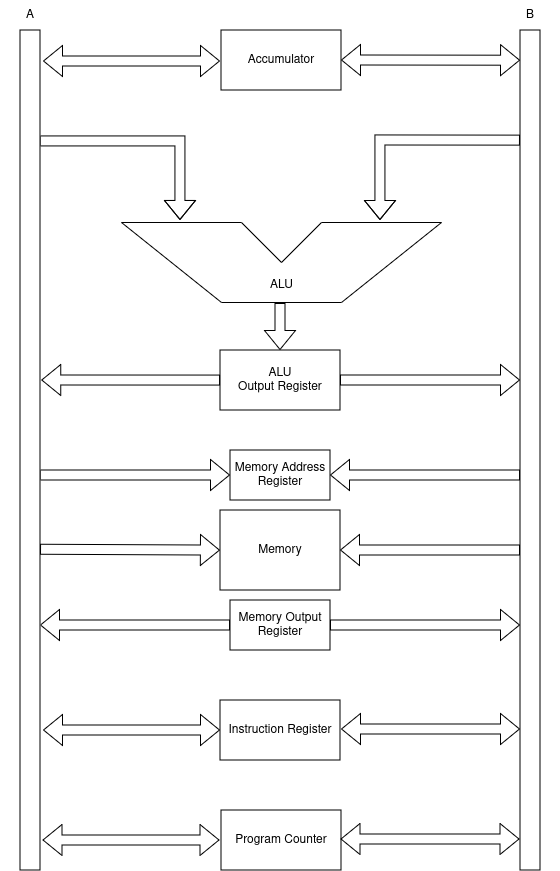
\includegraphics[scale=0.58]{img/Andromeda-Block Diagram.drawio}
\end{center}

\subsection{Instruction Flow}\label{subsec:state-machine-diagrams}
\par This section outlines the algorithm each instruction/addressing mode pair will execute.
The algorithm is laid out in terms of what steps will be executed for every rising and falling edge of the system clock.
Each step will correspond to a single micro-instruction.

\pagebreak
\subsubsection{\texttt{lda.imm}}
\subsubsection{\texttt{lda.dir}}
\subsubsection{\texttt{lda.rel}}
\subsubsection{\texttt{lda.off}}
\subsubsection{\texttt{lda.ind}}
\subsubsection{\texttt{lda.inc}}
\subsubsection{\texttt{lda.dec}}

\subsubsection{\texttt{sta.imm}}
\subsubsection{\texttt{sta.dir}}
\subsubsection{\texttt{sta.rel}}
\subsubsection{\texttt{sta.off}}
\subsubsection{\texttt{sta.ind}}
\subsubsection{\texttt{sta.inc}}
\subsubsection{\texttt{sta.dec}}

\subsubsection{\texttt{add.imm}}
\subsubsection{\texttt{add.dir}}
\subsubsection{\texttt{add.rel}}
\subsubsection{\texttt{add.off}}
\subsubsection{\texttt{add.ind}}
\subsubsection{\texttt{add.inc}}
\subsubsection{\texttt{add.dec}}

\subsubsection{\texttt{xor.imm}}
\subsubsection{\texttt{xor.dir}}
\subsubsection{\texttt{xor.rel}}
\subsubsection{\texttt{xor.off}}
\subsubsection{\texttt{xor.ind}}
\subsubsection{\texttt{xor.inc}}
\subsubsection{\texttt{xor.dec}}
